\chapter{Resultados}
\label{ch:resultados}
En este cap\'itulo se exponen resultados y an\'alisis de diferentes pruebas realizadas con la nueva versi\'on desarrollada del programa. La primera de las pruebas consiste en medir el desempe\~no de esta pipeline en t\'erminos de tiempo de ejecuci\'on y uso de memoria principal ocupada al procesar tres datasets (usados en el cap\'itulo \ref{ch:prev_work}) asociados a supernovas encontradas por HiTS\cite{hits}: SN14, SN18 y SN80. El segundo conjunto de experimentos corresponde al procesamiento sobre los 93 conjuntos de datos asociados a las supernovas encontradas por HiTS en el semestre de 2015. En ambos tipos de pruebas se busca comparar el rendimiento y los resultados del programa al emplear los diferentes filtros de Kalman implementados. Finalmente se muestran algunos resultados espec\'ificos obtenidos con el filtro unscented.
\bigskip


Para todas las experiencias se emple\'o umbrales de flujo y velocidad de flujo estimada de 200 [ADU] y 50 [ADU/d\'ia]. Adem\'as todas las im\'agenes procesadas poseen la misma dimensi\'on: $4094 \times 2046$ de alto por ancho, por lo que el campo \texttt{image\_size} de todos los filtros se configuraron en (4094, 2046). Por cada filtro se emplearon los siguientes valores de par\'ametros:

\subsection*{Filtro de Kalman B\'asico}
\begin{itemize}
\item \texttt{sigma\_a} : Se ocup\'o un valor de 0.1. Este valor se ajust\'o despu\'es de realizar diferentes pruebas variando este par\'ametro 100 y $10^{-4}$. Este t\'ermino es empleado durante el proceso de predicci\'on. 
\item \texttt{init\_var} : La varianza inicial de flujo y velocidad de flujo se estableci\'o con un valor de 100.0.
\item Se determin\'o 0.0 como valor inicial para las estimaciones de flujo y velocidad de flujo (estado).
\end{itemize}
\subsection*{Filtro de Kalman de m\'axima correntrop\'ia}
\begin{itemize}
\item \texttt{sigma\_a}: Se emple\'o valor 0.1. Este valor es usado, al igual que en el caso del filtro b\'asico, durante el proceso de predicci\'on (mismo m\'etodo).
\item \texttt{sigma}: Valor de la desviaci\'on est\'andar usado por defecto en caso de no usar optimizaci\'on de Silverman durante proceso de correcci\'on.
\item \texttt{silverman}: \texttt{False}. Para estas pruebas no se us\'o el m\'etodo de Silverman para obtener distribuci\'on ya que la implementaci\'on en el programa original se encuentra incompleta (por lo que una nueva implementaci\'on de esta funci\'on en el software desarrollado en este trabajo queda pendiente para trabajo futuro). 
\item \texttt{std\_factor}: Se estableci\'o como 100.0. Al no usarse el m\'etodo de Silverman, tampoco se hace uso de este valor.
\item \texttt{epsilon}: Se asign\'o valor de $10^{-6}$, como error m\'aximo. 
\item \texttt{max\_iter}: Se consider\'o 10 como n\'umero m\'aximo de iteraciones, que es el n\'umero definido por defecto (en el dise\~no del programa original).  
\item \texttt{init\_var} : La varianza inicial de flujo y velocidad de flujo se estableci\'o con un valor de 100.0.
\item Se determin\'o 0.0 como valor inicial para las estimaciones de flujo y velocidad de flujo (estado).

\end{itemize}
\subsection*{Filtro de Kalman Unscented}
\begin{itemize}
\item \texttt{f\_func:} Se defini\'o una funci\'on no lineal de grado 1.5 (informaci\'on entregada en \texttt{f\_args}).
\item \texttt{h\_func:} Se estableci\'o como la funci\'on identidad.
\item \texttt{f\_args:} El grado de la funci\'on se defini\'o como 1.5 y un factor de 1.0 (por tanto corresponde a la lista [1.5, 1.0]).
\item \texttt{h\_args:} Para estas pruebas se defini\'o como una lista vac\'ia ya que $h(\cdot)$ se trata de la funci\'on identidad.
\item \texttt{alpha:} Se estableci\'o como 0.001. Ya que con este valor se obtuvieron verdaderos positivos, aunque aumentaron los falsos positvos. A mayores valores disminuyen el n\'umero de candidatos encontrados (se probaron con valores de 0.0001 a 10).
\item \texttt{beta:} Se le asign\'o un valor de 2.0. Se asumi\'o distribuci\'on normal de las variables de estado\cite{matsinos}. 
\item \texttt{kappa:} Se le asign\'o un valor de 0.0. Se asumi\'o distribuci\'on normal de las variables de estado \cite{matsinos}.
\item \texttt{N:} Al tratarse de dos variables de estado, se establece \texttt{N}=2.
\item \texttt{sigma\_a}: Se defini\'o como 0.1. Se consider\'o usar el mismo valor para este par\'ametro de acuerdo a los resultados obtenidos con los filtros b\'asico y de m\'axima correntrop\'ia, ya que los resultados variaban negativamente (disminuyendo candidatos encontrados) al tomar valores (potencias de diez) mayores o menores a este n\'umero.    
\end{itemize}
Las condiciones iniciales del filtro unscented fueron diferentes a las definidas para los filtros b\'asico y de m\'axima correntrop\'ia. Esto debido a que la funci\'on no lineal depende de un $\Delta t$ medido desde cierta \'epoca $t_0$. Para estos experimentos se defini\'o $t_0$ como la primera \'epoca de observaci\'on (los otros m\'etodos dependen de la diferencia temporal entre una \'epoca y otra). Por tanto, se configur\'o el flujo inicial al valor del flujo calculado de la primera \'epoca. Adem\'as, la varianza del estado del flujo fue definida como la matriz de varianza de flujo calculado.


\section{Desempe\~no}
En esta secci\'on se describen los resultados obtenidos durante las experiencias de medici\'on de desempe\~no de la nueva versi\'on del programa en t\'erminos de tiempo y memoria principal usada. 
\bigskip

Las pruebas se realizaron usando el mismo conjunto de datos utilizado para medir el desempe\~no del programa original 
(Cap\'itulo \ref{ch:prev_work}), adem\'as se emplearon como herramientas de medici\'on igualmente el perfilador de memoria \texttt{mem\_profiler} y la librer\'ia \textsc{Resource}\footnote{M\'etodo \texttt{get\_rusage}}.

\subsection{Tiempo de ejecuci\'on}
Las Tablas \ref{tab:t7}, \ref{tab:t9} y \ref{tab:t11} muestran los resultados de tiempo medido en segundos de cada una de las partes del proceso de la rutina principal, para los tres datasets usando los filtros b\'asico, de m\'axima correntrop\'ia y unscented, respectivamente. 

\begin{table}[h!]
\centering
\caption{Tiempo de ejecuci\'on en segundos de cada proceso involucrado, usando el filtro de Kalman b\'asico refactorizado: c\'alculo de flujo, estimaci\'on de estados, detecci\'on de candidatos y guardado de candidatos resultantes en caso de haberlos. La \'ultima fila describe el tiempo promedio que toma por observaci\'on (en segundos igualmente) para cada uno de los procesos. }
\begin{tabular}{|l|r|r|r|r|}
\hline
\textbf{ID} & \textbf{C\'alc. Flujos [s]} & \textbf{Estim. KF [s]} &  \textbf{Detecci\'on [s]}  & \textbf{Obt. Candidatos [s]}\\ \hline \hline
SN14        & 297,93            & 28,36        &  33,53 & 0,00 \\ \hline
SN18            & 255,07             & 22,41         & 34,32  & 0,00\\ \hline
SN80            & 199,16             & 17,73         &   25,02 & 0,00 \\ \hline \hline
%Media & 303.08 &  26.23 & 37.83 & 0.01\\\hline 
$\bar{t}/Obs$ & 11,20 &  1,02 & 1,39 & 0,00\\\hline 
\end{tabular}
\label{tab:t7}
\end{table}

\begin{table}[h!]
\centering
\caption{Tiempo de ejecuci\'on en segundos de cada proceso involucrado, usando el filtro de Kalman de m\'axima correntrop\'ia refactorizado: c\'alculo de flujo de las im\'agenes, estimaci\'on de estado, detecci\'on de fuentes y guardado de candidatos. La \'ultima fila describe el tiempo promedio que toma por observaci\'on (en segundos) para cada una de las tareas.}
\begin{tabular}{|l|r|r|r|r|}
\hline
\textbf{ID} & \textbf{C\'alc. Flujos [s]} & \textbf{Estim. KF [s]} &  \textbf{Detecci\'on [s]}  & \textbf{Actual. Candidatos [s]}\\ \hline \hline
SN14        & 289,59            & 491,08        &  34,04 & 0,00 \\ \hline
SN18            & 256,95             & 437,37         &  33,00  & 0,00\\ \hline
SN80            & 199,98             & 346,98         &   24,96 & 0,00 \\ \hline \hline
%Media & 303.08 &  26.23 & 37.83 & 0.01\\\hline 
$\bar{t}/Obs$ & 11,00 &  19,06 & 1,38 & 0,00\\\hline 
\end{tabular}
\label{tab:t9}
\end{table}

\begin{table}[h!]
\centering
\caption{Tiempo de ejecuci\'on en segundos de cada tarea, usando el filtro de Kalman unscented: c\'alculo de flujo, estimaci\'on de filtros, detecci\'on de fuentes y guardado de candidatos. La \'ultima fila describe el tiempo promedio que toma por observaci\'on (en segundos) para cada uno de los procesos.}
\begin{tabular}{|l|r|r|r|r|}
\hline
\textbf{ID} & \textbf{C\'alc. Flujos [s]} & \textbf{Estim. KF [s]} &  \textbf{Detecci\'on [s]}  & \textbf{Actual. Candidatos [s]}\\ \hline \hline
SN14        & 280,67            & 342,88        &  123,68 & 0,01 \\ \hline
SN18            & 243,96             & 293,05         &  122,09  & 0,00\\ \hline
SN80            & 190,43             & 231,34         &   74,48 & 0,00 \\ \hline \hline
%Media & 303.08 &  26.23 & 37.83 & 0.01\\\hline 
$\bar{t}/Obs$ & 10,65 &  12,93 & 14,21 & 0,00\\\hline 
\end{tabular}
\label{tab:t11}
\end{table}
A todos estos resultados se les ha agregado la medici\'on de tiempo promedio por imagen (ya que las secuencias poseen largos diferentes). De estos resultados es posible deducir que el tiempo de c\'alculo de flujo por \'epoca siempre toma alrededor de 11.0 segundos. Esto es claro debido a que el proceso de c\'alculo de flujo es independiente del filtro escogido. Los tiempos de estimaci\'on de estado, por el contrario, var\'ian de filtro en filtro. Tomando mayor tiempo al usar el filtro de m\'axima correntrop\'ia. Sin embargo, opuesto a lo que se esperaba (ya que el proceso de detecci\'on ocurre una vez realizada la estimaci\'on de estado) el filtro unscented presenta un tiempo de detecci\'on casi diez veces mayor a los tiempos medidos en los otros filtros; esto se podr\'ia deber a las operaciones lineales realizadas durante el proceso de correcci\'on. 
\bigskip

Con los filtros b\'asico y de m\'axima correntrop\'ia no se encontraron candidatos en ninguno de los datasets. Sin embargo se detectaron candidatos con el filtro unscented al ejecutar la pipeline sobre los datos de la supernova SN14.
\bigskip

La totalidad y el promedio del tiempo que toma la ejecuci\'on de la pipeline con los tres filtros sobre los datasets se muestran en las Tablas \ref{tab:t8},  \ref{tab:t10} y \ref{tab:t12} (filtros b\'asico, de correntrop\'ia m\'axima y unscented, respectivamente).
\bigskip

\begin{table}[h!]
\centering
\caption{Tiempo de exploraci\'on (para detecci\'on de candidatos) usando filtro de Kalman B\'asico refactorizado. La \'ultima fila corresponde a tiempo total promedio por observaci\'on.}
\begin{tabular}{|l|r|}
\hline
\textbf{ID} & \textbf{Tiempo total [s]} \\ \hline
\hline
SN14  & 359,82 \\\hline
SN18  & 311,8\\\hline
SN80  & 241,91 \\\hline\hline
%Media & 367.15 & 374.83 & 741.98  \\\hline
 $\bar{t}/Obs. $& 13,61 \\\hline 
\end{tabular}
\label{tab:t8}
\end{table}


\begin{table}[h!]
\centering
\caption{Tiempo de exploraci\'on (para detecci\'on de candidatos) usando filtro de Kalman de m\'axima correntrop\'ia refactorizado. La \'ultima fila corresponde a tiempo total promedio por observaci\'on.}
\begin{tabular}{|l|r|}
\hline
\textbf{ID} & \textbf{Tiempo total [s]} \\ \hline
\hline
SN14  & 814,71 \\\hline
SN18  & 727,32\\\hline
SN80  & 571,92 \\\hline\hline
%Media & 367.15 & 374.83 & 741.98  \\\hline
 $\bar{t}/Obs. $& 31,58 \\\hline 
\end{tabular}
\label{tab:t10}
\end{table}

\begin{table}[h!]
\centering
\caption{Tiempo de exploraci\'on (para detecci\'on de candidatos) usando filtro unscented. La \'ultima fila corresponde a tiempo total promedio por observaci\'on en segundos.}
\begin{tabular}{|l|r|}
\hline
\textbf{ID} & \textbf{Tiempo total [s]} \\ \hline
\hline
SN14  & 747,24 \\\hline
SN18  & 659,1\\\hline
SN80  & 496,25 \\\hline\hline
%Media & 367.15 & 374.83 & 741.98  \\\hline
 $\bar{t}/Obs. $& 28,32 \\\hline 
\end{tabular}
\label{tab:t12}
\end{table}

De los resultados expuestos sobre el tiempo total de ejecuci\'on se desprende que la pipeline demora menos con el filtro b\'asico, mientras que con el de m\'axima correntrop\'ia es con el que m\'as se demora.

\subsection{Uso de memoria}
Las Figuras \ref{fig:mem_new_kbf}, \ref{fig:mem_new_mcc} y \ref{fig:mem_ukf} muestran el comportamiento del consumo de memoria al usar la nueva versi\'on del filtro b\'asico, de m\'axima correntrop\'ia y el nuevo filtro unscented, respectivamente, ejecutando la pipeline refactorizada sobre los tres conjuntos de datos (SN14, SN18 y SN80). 

\begin{figure}[h!]
\centering
\subfloat[Memoria ocupada en SN14]{\label{fig:new_kbf_14}{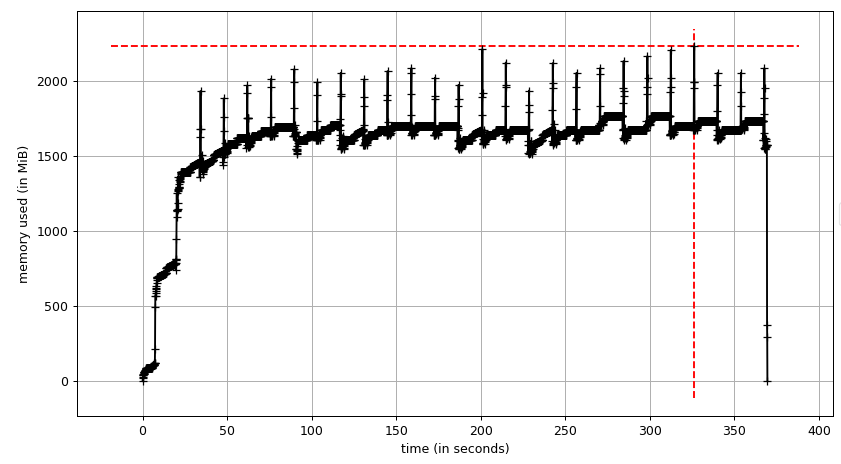
\includegraphics[width=0.5\textwidth]{images/results/sn14_new_bk}}}\hfill
\subfloat[Memoria ocupada en SN18]{\label{fig:new_kbf_18}{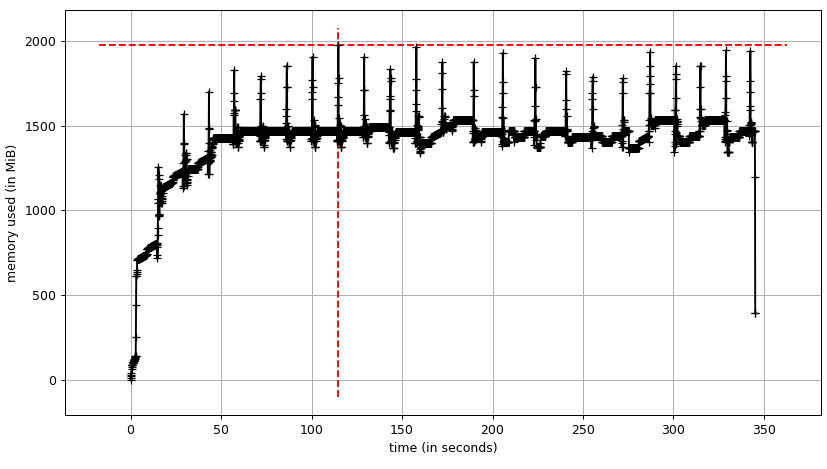
\includegraphics[width=0.5\textwidth]{images/results/sn18_new_bk}}}\vfill
\subfloat[Memoria ocupada en SN80]{\label{fig:new_kbf_80}{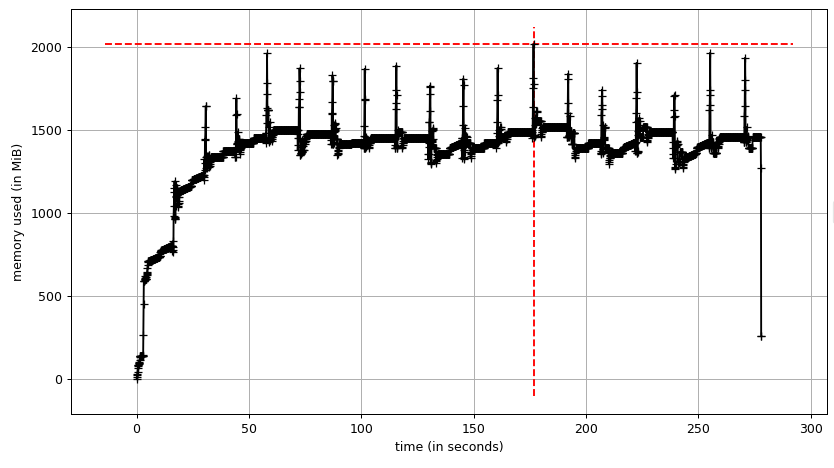
\includegraphics[width=0.5\textwidth]{images/results/sn80_new_bk}}}
\caption{Comportamiento de la memoria (en mebibytes) durante la ejecuci\'on para los tres conjuntos de datos usando el filtro de Kalman B\'asico.}
\label{fig:mem_new_kbf}
\end{figure}

De la Figura \ref{fig:mem_new_kbf} se desprenden los m\'aximos alcanzados durante cada ejecuci\'on con el filtro b\'asico. Los resultados en megabytes se listan en la Tabla \ref{tab:mem3}.
\pagebreak

\begin{table}[h!]
\centering
\caption{Memoria principal (en unidades de MB) usada durante la ejecuci\'on del programa refctorizado usando filtro de Kalman B\'asico.}
\begin{tabular}{|l|r|}
\hline
\textbf{ID} & Memoria [MB]\\\hline\hline
SN14 & 2347,78\\\hline
SN18 & 2254,93\\\hline
SN80 & 2365,07\\\hline
\end{tabular}
\label{tab:mem3}
\end{table}


\begin{figure}[h!]
\centering
\subfloat[Memoria ocupada en SN14]{\label{fig:new_mcc_14}{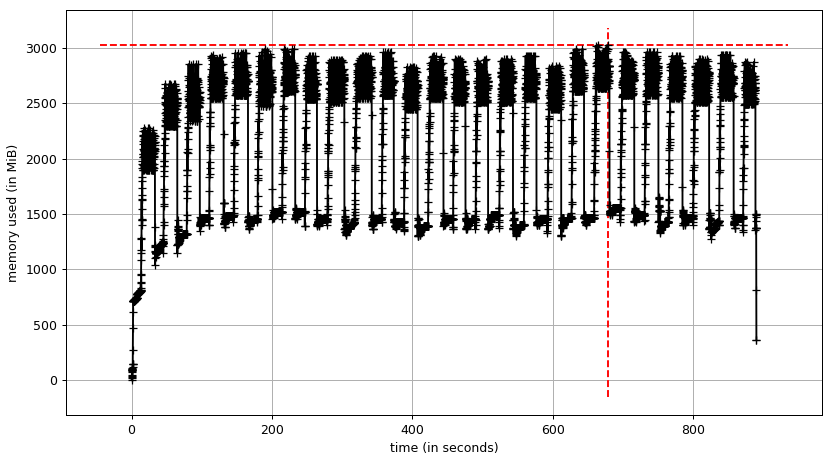
\includegraphics[width=0.5\textwidth]{images/results/sn14_new_mcc}}}\hfill
\subfloat[Memoria ocupada en SN18]{\label{fig:new_mcc_18}{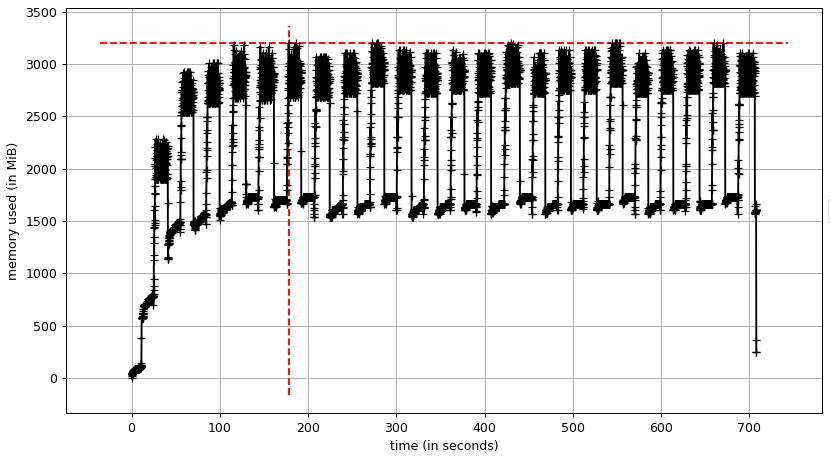
\includegraphics[width=0.5\textwidth]{images/results/sn18_new_mcc}}}\vfill
\subfloat[Memoria ocupada en SN80]{\label{fig:new_mcc_80}{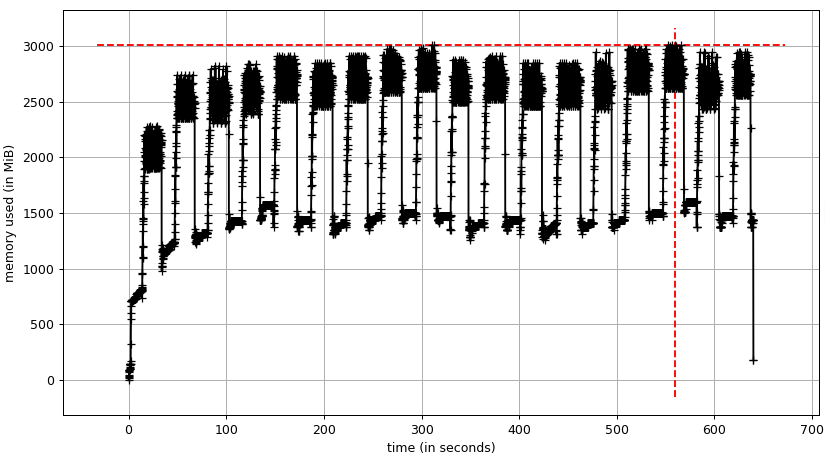
\includegraphics[width=0.5\textwidth]{images/results/sn80_new_mcc}}}
\caption{Comportamiento de la memoria (en mebibytes) durante la ejecuci\'on para los tres conjuntos de datos. En los tres lanzamientos se us\'o el filtro de Kalman de m\'axima correntrop\'ia.}
\label{fig:mem_new_mcc}
\end{figure}

De las series mostradas en la Figura \ref{fig:mem_new_mcc} se obtienen los m\'aximos alcanzados de memoria principal ocupada al utilizar el filtro de m\'axima correntrop\'ia listados en la Tabla \ref{tab:mem4}. 
\bigskip

\begin{table}[h!]
\centering
\caption{Memoria principal (en unidades de MB) usada durante la ejecuci\'on del programa refactorizado usando filtro de Kalman de m\'axima correntrop\'ia.}
\begin{tabular}{|l|r|}
\hline
\textbf{ID} & Memoria [MB]\\\hline\hline
SN14 & 3359,54\\\hline
SN18 & 3350,53\\\hline
SN80 & 3330,93\\\hline
\end{tabular}
\label{tab:mem4}
\end{table}

\begin{figure}[h!]
\centering
\subfloat[Memoria ocupada en SN14]{\label{fig:ukf_sn14}{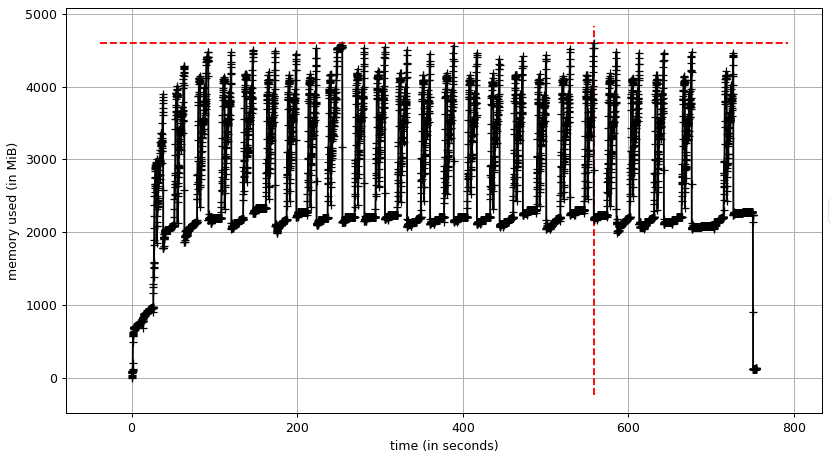
\includegraphics[width=0.5\textwidth]{images/results/sn14_ukf}}}\hfill
\subfloat[Memoria ocupada en SN18]{\label{fig:ukf_sn18}{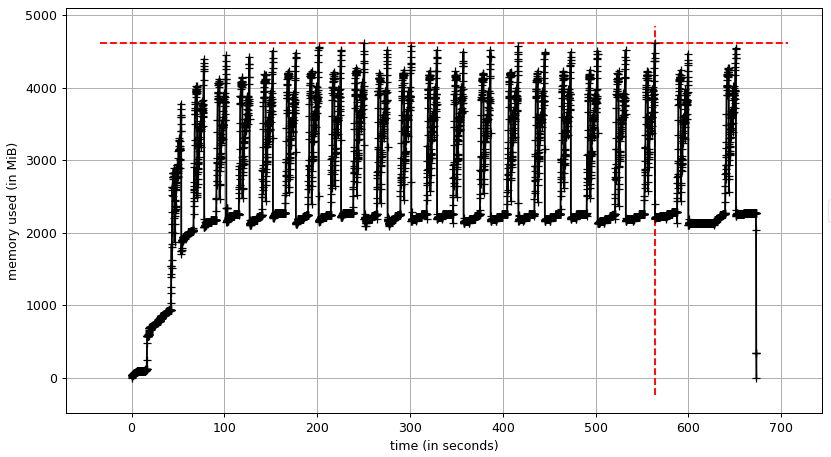
\includegraphics[width=0.5\textwidth]{images/results/sn18_ukf}}}\vfill
\subfloat[Memoria ocupada en SN80]{\label{fig:ukf_sn80}{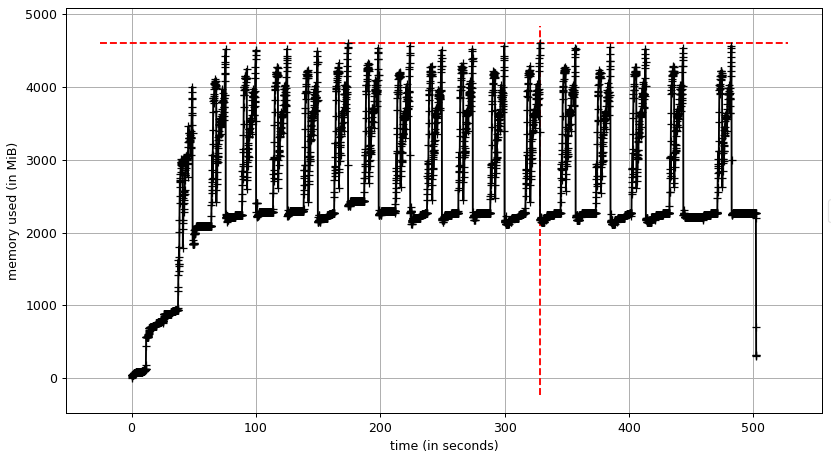
\includegraphics[width=0.5\textwidth]{images/results/sn80_ukf}}}
\caption{Comportamiento de la memoria (en mebibytes) durante la ejecuci\'on para los tres conjuntos de datos. En los tres lanzamientos se us\'o el filtro de Kalman unscented.}
\label{fig:mem_ukf}
\end{figure}

Los m\'aximos de uso de memoria principal al emplear el filtro unscented, para cada conjunto de datos, se muestra en la Tabla \ref{tab:mem5}.

\begin{table}[h!]
\centering
\caption{Memoria principal (en unidades de MB) usada durante la ejecuci\'on del programa refactorizado usando filtro de Kalman unscented.}
\begin{tabular}{|l|r|}
\hline
\textbf{ID} & Memoria [MB]\\\hline\hline
SN14 & 4827,82\\\hline
SN18 & 4835,96\\\hline
SN80 & 4821,89\\\hline
\end{tabular}
\label{tab:mem5}
\end{table}

Los resultados de memoria principal muestran un uso intensivo de esta al usar el filtro unscented. Esto puede ser debido a la serie de operaciones lineales que se debe realizar al momento de predecir y corregir. Tambi\'en se desprende que el uso de memoria es menor con el filtro b\'asico.
\bigskip
 
\section{Detecci\'on}
En esta secci\'on se exponen los resultados obtenidos al procesar los datos de las 93 supernovas con los tres filtros implementados. En particular se muestran las cantidades de verdaderos positivos, falsos negativos, falsos positivos y el n\'umero de conjunto de datos que no pudieron ser procesados por no contar con alg\'un tipo de imagen o archivo necesario para su procesamiento (en este caso, fue la falta de im\'agenes de diferencia). Se considera como falso positivo todo aquello que no est\'e catalogado como supernova de acuerdo a HiTS; es decir, estrellas variables u otro tipo de objetos celestes, rayos c\'osmicos, junto a ruido en la intensidad de los p\'ixeles, etc.
\bigskip

Los par\'ametros usados por cada filtro son los mismos descritos al inicio de este cap\'itulo.

\subsection{Filtros b\'asico y de m\'axima correntrop\'ia}
La Tabla \ref{tab:tpfn_new} muestra los resultados obtenidos con la nueva versi\'on de la pipeline, empleando los filtros refactorizados b\'asico y de m\'axima correntrop\'ia.
\bigskip

\begin{table}[h!]
\centering
\caption{N\'umero de verdaderos positivos (TP), falsos negativos (FN) y falsos positivos (FP) encontrados usando cada uno de los filtros en el conjunto de datos de HiTS. La cuarta columna de valores muestra la cantidad de conjuntos de datos que no pudieron ser procesados.}
\begin{tabular}{|l|r|r|r|r|}
\hline
\textbf{Filtro} & \textbf{TP} & \textbf{FN} & \textbf{FP} & \textbf{NaN}\\ \hline
Básico          & 36          & 54          & 37 &  3 \\ \hline
M\'ax. Corr.             & 36          & 54          & 40  & 3 \\ \hline
\end{tabular}
\label{tab:tpfn_new}
\end{table}
\bigskip

De la Tabla \ref{tab:tpfn_new} se obtiene que el filtro de m\'axima correntrop\'ia encuentra la misma cantida de supernovas conocidas que el filtro b\'asico, y detecta m\'as falsos positivos. Sin embargo cabe recalcar que para esta experiencia no se us\'o el m\'etodo de Silverman para estimar $\sigma$ en el proceso de correcci\'on, por lo que podr\'ia existir opciones de mejora.
\bigskip

De acuerdo a la Tabla \ref{ap:tab1}, Ap\'endice \ref{ap:pip_ref} varias de las detecciones ocurren despu\'es  del per\'iodo de alta cadencia (despu\'es de MJD 57075.00) y pr\'acticamente no hay diferencia entre ambos filtros. Lo primero puede deberse a que es necesario cumplir las condiciones mencionadas en el cap\'itulo \ref{ch:refactoring}, secci\'on \ref{sec:detec} en la clase \textsc{SourceFinder} por cuatro \'epocas consecutivas para emitir una alerta. Por otro lado otras detecciones realizadas por ambos filtros ocurrieron en un per\'iodo bastante alejado del intervalo de alta cadencia, por lo que el distanciamiento entre las observaciones puede haber favorecido a la detecci\'on.
\bigskip
  

\subsection{Filtro unscented}
Con el filtro unscented se realizaron dos pruebas. En ambos casos se asumi\'o la funci\'on $h(\cdot)$ como la funci\'on identidad. En cambio la funci\'on $f(\cdot)$ tom\'o dos formas no lineales en funci\'on de $\Delta t$: $f(\Delta t) = (\Delta t)^{1.5}$ y $f(\Delta t) = (\Delta t)^{2}$. Los resultados obtenidos para verdaderos positivos y falsos positivos y negativos se muestran en la Tabla \ref{tab:tpfn_ukf}.

\begin{table}[h!]
\centering
\caption{N\'umero de verdaderos positivos (TP), falsos negativos (FN) y falsos positivos (FP) encontrados usando el filtro unscented para dos tipos de funciones no lineales: $f(\Delta t) = (\Delta t)^{1.5}$ y $f(\Delta t) = (\Delta t)^{2}$. La tercera columna de valores muestra la cantidad de conjuntos de datos que no puedieron ser procesados.}
\begin{tabular}{|l|r|r|r|r|}
\hline
\textbf{Filtro} & \textbf{TP} & \textbf{FN} & \textbf{FP} & \textbf{NaN}\\ \hline
$\Delta t^{1.5}$          & 2          & 87          & 110 &  3 \\ \hline
$\Delta t^{2}$             & 3          & 87          & 108  & 3 \\ \hline
\end{tabular}
\label{tab:tpfn_ukf}
\end{table}
\bigskip

Se observa que bajo la configuraci\'on seleccionada de valores de par\'ametros, el desempe\~no de la detecci\'on es bastante pobre. No obstante se debe considerar la posibilidad de mejorar este resultado estudiando condiciones iniciales, valores de par\'ametros y en particular, las funciones a utilizar ($f(\cdot)$ y $h(\cdot)$).
\bigskip

Para observar si el filtro unscented est\'a trabajando como se espera, es posible visualizar que est\'a sucediendo con las estimaciones y los valores de flujo con alguna de sus detecciones. Se seleccion\'o una de las supernovas encontradas por este filtro en el CCD N2, campo 7 usando una funci\'on $f(\Delta t) = \Delta t^{2}$.

\begin{figure}
\centering
\includegraphics[scale=0.5]{/home/paloma/Documents/Memoria/results/RESULTS/lc_sem_15A_field_07_ccd_N2_obj_0.png}
\caption{En la primera gr\'afica de arriba hacia abajo se muestra el comportamiento del flujo medido y el flujo predicho y estimado. En esta representaci\'on se observa que el flujo se dispara a partir de la fecha 57075. De la misma forma, se dispara las velocidades de flujo estimado y predicho de acuerdo al segundo gr\'afico. El siguiente siquiente esquema indica el crecimiento de flags de invalidez de los p\'ixeles  mientras que la \'ultima imagen da cuenta del r\'apido crecimiento de las varianzas y covarianzas de estimaci\'on y predicci\'on de las variables de estado. }
\label{ukf_rlc}
\end{figure}

\begin{figure}
\centering
\includegraphics[scale=0.5]{/home/paloma/Documents/Memoria/results/RESULTS/stamps_sem_15A_field_07_ccd_N2_obj_0.png}
\caption{Representaci\'on en p\'ixeles de lo que sucede con el flujo observado, las estimaciones y los flags de los p\'ixeles. Se distingue la saturaci\'on sobre las matrices de flujo y velocidad estimada.}
\label{ukf_stamp}
\end{figure}

\begin{figure}
\centering
\includegraphics[scale=0.5]{/home/paloma/Documents/Memoria/results/RESULTS/space_states_sem_15A_field_07_ccd_N2_obj_0.png}
\caption{Se observa el comportamiento conjunto del flujo y velocidad estimados. El r\'apido crecimiento de ambas variables es bastante notable}
\label{ukf_rss}
\end{figure}

De acuerdo a las Figuras \ref{ukf_rlc}, \ref{ukf_stamp} y \ref{ukf_rss} uno de los problemas que adolece este filtro es el de crecimiento r\'apido, por lo que de alguna forma se debe contrarrestar esta gran alza trabajando,  tal vez, sobre la funci\'on de predicci\'on $f(\cdot)$.

\section{Observaciones}
Respecto de las detecciones obtenidas con los filtros b\'asico y de m\'axima correntrop\'ia tanto para esta versi\'on como para la original, se detectaron el mismo  n\'umero de supernovas: treinta y seis. Sin embargo disminuyeron notablemente los falsos positivos respecto de la versi\'on orignal. Esto \'ultimo se piensa puede deberse a un nuevo ordenamiento y filtrado m\'as precisos de los archivos necesarios para ejecutar la rutina.
\bigskip

Por otro lado en t\'erminos de desempe\~no, si bien la nueva versi\'on ha podido disminuir tiempos de ejecuci\'on, a\'un no se logra disminuir la cantidad de memoria principal usada respecto del programa antecesor.  
